\chapter{Developing the tool}
This chapter details how the visualization tool was built.

\section{Creating the tiles}
The tiles were created using a modified version of gdal2tiles, which was changed to create tiles following the XYZ format. However, since the default output bit depth is too low, it would have to be modified further. The file format would also have to be changed to tiff in order to be visualized with the geotiff.js library. 

\subsection{Changing the file type}
Changing the file format can be done by changing two lines in the gdal2tiles script:

\begin{lstlisting}[language=iPython, caption={Changing the file format}, label= VoresPY,escapechar=|]
#Original code
#self.tiledriver = 'PNG'
#self.tileext = 'png'
#New code
self.tiledriver = 'GTiff'
self.tileext = 'tiff'
\end{lstlisting}
This changes the raster driver from png to the geotiff format and the file extension from png to tiff. 
\citep{RasterDrivers}
The geospatial information, which is the difference between a geotiff and a regular tiff, gets lost in process. This information is not important for this project since the tiles are being loaded based on their name and folder placement, not based on the internal metadata.

Running gdal2tiles with these changes will produce a tiff file, which still would be limited to 8 bits. 
\subsection{Increasing the bit depth}
The reason for the bit limit is that gdal2tiles uses the memory dataset driver, which have 8 bits as default.  This default can overwritten to 32 bits by adding “gdal.GDT\_Int32” to every instance where the driver is being used as demonstrated in code x. 
\citep{MoreThan8}

\begin{lstlisting}[language=iPython, caption={Increasing the bit depth}, label= VoresPY,escapechar=|]
self.mem_drv = gdal.GetDriverByName('MEM')
...
#Old code
#dstile = mem_drv.Create('', tile_size, tile_size, tilebands)
#New code
dstile = self.mem_drv.Create('', self.tilesize, self.tilesize, tilebands, gdal.GDT_Int32)
\end{lstlisting}
The memory driver is being used four times, which all have been changed in a similar fashion.


The script is now generating tiff tiles correctly. However it also generates KML files for visualization in Google Earth, which is undesired since it would increase the processing time and required storage space. 
\subsection{Prevent generation of Google Earth files}
gdal2tiles is automatically generating KML files if the projection is EPSG:4326. According to the documentation for the official gdal2tiles this can be disabled with the command "--no.kml".
\citep{gdal2tilesDoc}


This command does not prevent the creation of the files in the modified version. Therefore the automatic generation has been removed from the code. This was done by commenting out the lines shown in x. 

\begin{lstlisting}[language=iPython, caption={Increasing the bit depth}, label= KML,escapechar=|]
 if self.out_srs and srs4326.ExportToProj4() \
         == self.out_srs.ExportToProj4():
     self.kml = True
     self.isepsg4326 = True
     if self.options.verbose:
         print('KML autotest OK!')
\end{lstlisting}
        

\fxnote{Write about the addition to time the whole thing}


\subsection{Command for tile creation}

After all the modification are in place the script can be run by running the command illustrated below:


python <path to modified gdal2tiles script> --leaflet --zoom=<desired zoom levels> --profile=raster --webviewer=none <input file> <output directory>


Most of these inputs are from the documentation for the original gdal2tiles, though the leaflet command is from the modified version. This command ensures that tiles are being created following the XYZ formatting instead of the TMS. The zoom command defines which zoom levels should be generated. An example of an input could be 0-2, which would generate tiles for the zoom levels 0, 1 and 2. 

Setting the profile to raster was done because the two other options (mercator and geodetic) resulted in the error message "list index out of range", while the raster profile gave a useable product. The selection of this options and its consequences is expanded upon in section x.  

The webviewer option prevent the generation of webviewers to visualize the tiles. These default webviewers is created to visualize tiles of the original format, so they would be unable to visualize the modified tiles. 
The input file is the name of the processed file and output directory is the folder, where the tiles get created. 
\subsection{Result}

While creating the tiles the error message "ERROR 1: Buffer too small" gets displayed. The tiles are still being generated with the correct formatting and bit depth. This is an error message from numpy, which gdal2tiles are using. 
\citep{MoreThan8}
The generated tiles appears as they should, so this error message is potentially referring to the geospatial information, which gets lost.

The tiles at the rightmost and bottom edges have an edge as shown in figure x. This edge is not being shown, when the tile is being loaded into the map. A comparison between the input file and the tile shows that all data is being displayed. The bottom part of the input file is the last part before the edge. This edge seems to be generated because the input file was not perfectly dividable with the tile size as illustrated in figure x.
https://github.com/ARiisgaard/Thesis/issues/22
This edge could be another explanation for the error message. 



\fxnote{Make figures - remove link}


\fxnote{Test if normal gdal2tiles tiles have edges - if false, then point it out here}

The script also produces an xml file with metadata. An example of the content of said metadata file can be seen in code x.

\begin{lstlisting}[language=HTML5, caption={The metadata from the xml file generated by the modified gdal2tiles}, label= VoresHTML,escapechar=|]
<?xml version="1.0" encoding="UTF-8"?>
<TileMap tilemapservice="http://tms.osgeo.org/1.0.0" version="1.0.0"><Abstract/><SRS>GEOGCS["WGS 84",DATUM["WGS_1984",SPHEROID["WGS 84",6378137,298.257223563,AUTHORITY["EPSG","7030"]],
AUTHORITY["EPSG","6326"]],PRIMEM["Greenwich",0,AUTHORITY["EPSG","8901"]],UNIT["degree",0.0174532925199433,
AUTHORITY["EPSG","9122"]],AXIS["Latitude",NORTH],AXIS["Longitude",EAST],AUTHORITY["EPSG","4326"]]
</SRS><BoundingBox maxy="25.00000000000814" maxx="80.99999999999989" miny="19.00000000000815" minx="72.99999999999989"/><Origin y="19.00000000000815" x="72.99999999999989"/><TileFormat extension="tiff" mime-type="image/tiff" height="256" width="256"/><TileSets profile="raster"><TileSet order="2" units-per-pixel="0.00833333333333" href="2"/><TileSet order="3" units-per-pixel="0.00416666666667" href="3"/><TileSet order="4" units-per-pixel="0.00208333333333" href="4"/><TileSet order="5" units-per-pixel="0.00104166666667" href="5"/><TileSet order="6" units-per-pixel="0.00052083333333" href="6"/><TileSet order="7" units-per-pixel="0.00026041666667" href="7"/><TileSet order="8" units-per-pixel="0.00013020833333" href="8"/><TileSet order="9" units-per-pixel="0.00006510416667" href="9"/></TileSets></TileMap>
\end{lstlisting}

\section{Processing time}

\begin{figure} [H]
	\centering
	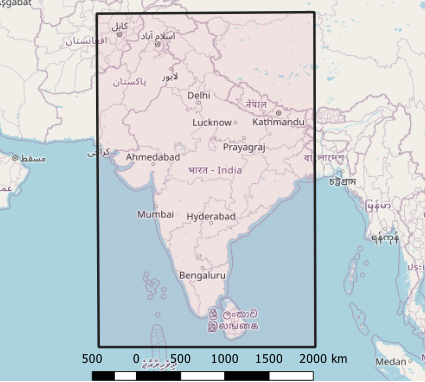
\includegraphics[width=.8\textwidth]{Pictures/ProcessingTime}
	\caption{Illustration of the area used for timing the tile generation}
	\label{ProcessingTime}
\end{figure}

The processing time is tested using the area of India shown in figure \citep{ProcessingTime}. This polygon with a 9 291 842 km$^2$ area was processed into tiles for each zoom level between 0 to 9. This is the equivalent of 349525 tiles as calculated with the formula presented in section x. 
\begin{equation}
2^{2n}
2^{2*9}+2^{2*8} .. . 2^{2*0} = 349525 tiles
\end{equation}
The creation of these tiles took 6 hours and 4 minutes. The amount of time mainly depends on the highest zoom level, since the number of tiles in a layer get quadrupled whenever the zoom level increases. In comparison the same area at the zoom levels 0-7 only took 22 minutes.

This processing time is not ideal, but it can theoretically be shortened with multiprocessing.
\subsection{Parallel processing of tiles}
Multiprocessing is the usage of multiple of the computer’s processors. Python is by default only able to use a single processor, even if multiple are available.  This can be circumvented with the multiprocessing module.
%Must not be reliant on previous outcomes
%Does not need to be executed in a particular order
%Does not return anything that would need to be accessed later in the code
\citep{Multiprocessing}
The modified version by \citet{gdalLeaflet} also has a multiprocessing version allowing each processer of the computer to work separately on generating tiles. However, the task is not properly distributed between the processes. This means that not all of the tiles are being generated. 
\citep{NoMulti}
Therefore, the slower single process version has been used for this project.


\section{Visualizing tiles}
After the tiles are created, they are stored in a folder, which is uploaded to the testserver along the index file. 
The metadata from the xml file must be loaded into the map to be able to visualize the tiles. Normally this could be done using the WMTSCapabilities() function in Openlayers.
\citep{WmtsOl}
However, the formatting of the xml file produced by gdal is different from the format, which this function can read. Therefore, a small script has been created to parse the xml file and store the information in a metadata object. This object, tileMetadata, stores the bounding box, origin, center coordinates as well as tilesize. The initial version of the object also stored the resolution data, which is called units-per-pixel in code x. This led to some inconsistency when loading tiles, that had been generated without some of the lower zoom level. This will be further expanded upon in section x. Therefore, the resolution was instead generated using the script x, where 0.0333 is the value for units-per-pixel at zoom level 0. 

\begin{lstlisting}[language=JavaScript, caption={The JavaScript in the project}, label= VoresJS,escapechar=|]
for (var z = 0; z < 14; ++z) {
// generate resolutions and matrixIds arrays for this WMTS
//The number in the resolution calculation is the units-per-pixel value at zoomlayer 0 in the xml file generated by gdal2tiles
resolutions[z] = 0.03333333333514 / Math.pow(2, z);
matrixIds[z] = z;
}
\end{lstlisting}
Using this metadata, the tiles could be visualized using the olGeoTiff class. 

%\begin{lstlisting}[language=JavaScript, caption={The JavaScript in the project}, label= VoresJS,escapechar=|]
%var wmslayer = new ol.layer.Tile({
%  source: new ol.source.WMTS({
%    url: tileFolders + '/{TileMatrix}/{TileCol}/{TileRow}.tiff',
%    projection: projection,
%    tileGrid: new ol.tilegrid.WMTS({
%      origin: tileMetadata[origin],
%      resolutions: resolutions,
%      matrixIds: matrixIds,
%      tileSize: tileMetadata[tileSize],
%    }),
%    requestEncoding: 'REST',
%    transition: 0
%  }),
%  extent: tileMetadata[boundingBox],
%  opacity: 0.65 
%});
%var olgt_map = new olGeoTiff(wmslayer);
%\end{lstlisting}


\subsection{Custom colors scheme}
Using colorbrewer a custom sequential colorscheme was generated. This scheme was added to Plotty and selected as a color palette.
\fxnote{This code might change a bit, so wait with writing}


\section{Loading data at a wrong resolution}\label{PresentingBug}

Figure \ref{MapWithWrongResolution} shows how the map looked, when the tiles are visualized. 
\fxnote{Rewrite this with new knowledge}

\begin{figure} [H]
	\centering
	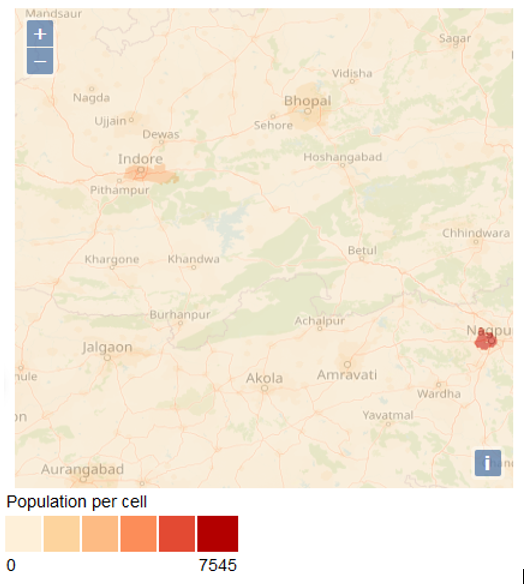
\includegraphics[width=.8\textwidth]{Pictures/MapWithWrongResolution}
	\caption{The map is looking correct, but with tiles from the wrong zoom level}
	\label{MapWithWrongResolution}
\end{figure}


While the map appeared to look alright, it was loading tiles from the wrong zoom level. The tiles always got loaded from a zoom level three levels higher than intended. So the map in figure \ref{MapWithWrongResolution} is visualizing the map at zoom level 7, but loading and displaying tiles from zoom level 2. It was not possible to force the map to load tiles from a different zoom level.

Some experiments with loading tiles from the current view and zoom level 7 crashed the map with the error message “Insufficient Resources”. The amount of loaded tiles seems unnecessarily high and size of the tiles too small. This seems to indicate, that the tiles, which the modified version of gdal2tiles associates with zoom level 7 in fact belongs to a higher zoom level.

In figure \ref{DifferentZoom} these different zoom levels have been illustrated. The expected zoom level, which Openlayer

The Displayed zoom level (DZL) is the tiles, that are being loaded and visualised in Openlayers. The expected zoom level (EZL) is the zoom level, which Openlayers is displaying the map in. However as mentioned earlier there are too many tiles to load, when using this zoom level and map extent. The coloring should therefore ideally be done based on a zoom level between these two zoom levels. This zoom level have been defined as the intended zoom level (IZL).

\begin{figure} [H]
	\centering
	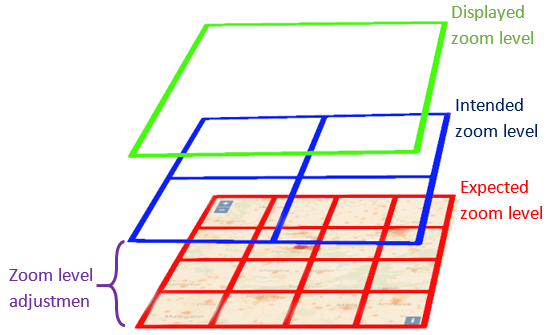
\includegraphics[width=.8\textwidth]{Pictures/DifferentZoom}
	\caption{An overview of the differences in zoom levels, which the map is displayed at (red), the displayed tiles get loaded in (green) and the zoom level, which should have been displayed (blue). The zoom level adjustment is the difference between the Expected and Intended zoom level}
	\label{DifferentZoom}
\end{figure}
\fxnote{Explain the need for zoom level 0 better}
This issue was not fixed, but theories behind the origin of it is discussed in section x. When the resolution data was gathered from the metadata file, the difference between the loaded and the actual zoom level would between different sets of tiles. This variance would depend on the which zoom levels were not being generated. So, if only the zoom levels 2-7 were generated, the difference would increase by one for each missing layer. In this case the loaded tiles would instead be wrong by 5, calculated as the default wrongness of 3 plus 2 for missing zoom layer 0 and 1. 
This bug will be defining for the rest of the code.



\section{Calculate max value in current extent}
Calculating the highest value in the current extent can be divided into two smaller tasks. Figuring out which tiles currently are being displayed and processing these tiles. It was decided not to calculate the lowest value in each tiles, since the calculation increased the processing time without yielding any benefit. This is expanded upon in section \ref{WhyNoMin}

\fxnote{min values have been removed earlier, right? No need to mention them here too}
\subsection{Current displayed tiles}\label{CurrentDisplayedTiles}

The tiles, which currently is within the view, can be found using the Openlayers tileGrid method forEachTileCoord. This method can trigger a function for each tile coordinate within a given zoom level and extent. 
\citep{forEachTileCoord}
These tile coordinates can then be translated to the tile name and folder location using getTileUrlFunction.
%The method is going through the tiles based on their coordinates, but this can be translated to the tile urls using the getTileUrlFunction.
\begin{lstlisting}[language=JavaScript, caption={}, label= VoresJS,escapechar=|]
var tileUrlFunction = wmslayer.getSource().getTileUrlFunction()
var zoomlevelAdjustment = 3
wmslayer.getSource().getTileGrid().forEachTileCoord(loadExtent, mapZoom - zoomlevelAdjustment, function(tileCoord) {
	tileName = tileUrlFunction(tileCoord, ol.proj.get('EPSG:4326'))
	maxValueInTile()
}
\end{lstlisting}
If the function is just given the zoom level of the map it will trigger for the tiles in the Expected Zoom Level. This would not work, since there are too many tiles in this level with the current extent. Instead the function is used with the Intended Zoom Level, which is calculated as the Expected Zoom Level minus a zoom level adjustment. Using an adjustment value of 3 was found to give a responsive user experience.

% This means that it on zoom level 7 would load the tiles, that should be rendered on zoom level 7. Due to the issue mentioned section \ref{PresentingBug} it is not the tiles from that zoom level, which are being displayed. Instead the tiles from zoom level 2 are being displayed. This will complicate some of the next steps. 
%The adjustment to the zoom level is in order to load the tiles, which should have been displayed.

\subsection{Max value for each tile}
If the tiles added to the map had been from the Intended Zoom Level, then the max value of a tile could have been calculated as olGeoTiff was running. olGeoTiff already holds the values for the tiles in a dataarray, so finding the maximum value could be done with a single line adding a tiles max value to the object for that tile. %This line is shown in code x, where urlToTiff is the name of the object, which holds the data.

%maxValueTileData[url].maxValue = Math.max(...urlToTiff[url][0])

However, since olGeoTiff holds data from an incorrect zoom layer this does not function. A possible solution would be to trigger forEachTileCoord for the Displayed Zoom Level. This solution was not implemented since the tiles from the Displayed Zoom Level are so large, that they would show data outside the view of the map. This means that the coloring could be based on the information that was outside of the current view.

The alternative solution is to run another function going through the tiles, which should have been displayed and find the highest value among these. This results in a map where the tiles from the Displayed zoom level were being colored based on information from the tiles at the Intended zoom level. This solution is by no means ideal. It means requesting tiles from two layers, one for displaying on the map a one for calculating the relevant max values. Loading more data than necessary will make the script slower, but since no better solution was found this have been implemented.

The calculation of the maximum value for each tile was done in a very similar fashion to how olGeoTiff operates as illustrated in figure \ref{CalculateMaxValue}. An object holds information about all tiles, which have been processed and the max value is known. When the function is run for a tile it first checks if the tile already has been processed. If that is not the case, then it will create an object for the data, which it then will load and parse with geotiff.js. %The data array with parsed data will then be run through as descripted in code x to calculate the maximum value. 
This maximum value will then be returned to the map. 

\fxnote{Write about combining my object with his object - would result in it not having to open the same raster twice, in case of zooming}
\begin{figure} [H]
	\centering
	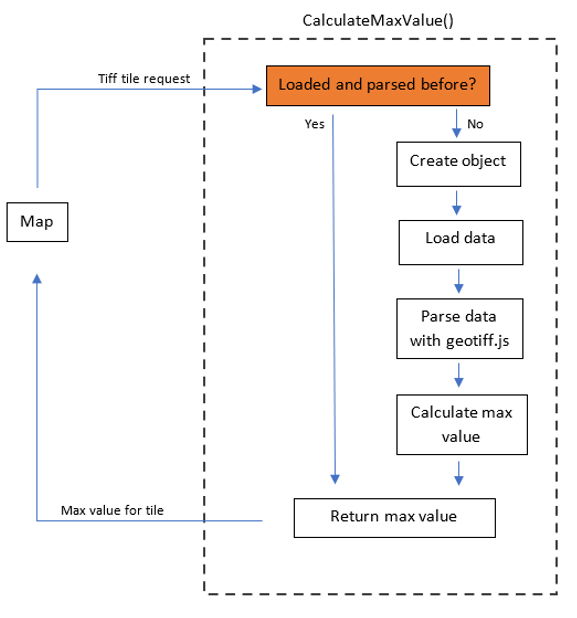
\includegraphics[width=.8\textwidth]{Pictures/CalculateMaxValue}
	\caption{Flow diagram of the calculation over max value in a tile}
	\label{CalculateMaxValue}
\end{figure}



\subsection{Highest tile value currently displayed}


To find the largest tile value among all the currently displayed tiles forEachTileCoord is used. forEachTileCoord does not have a trigger for when it has run through all the tiles. This functionality is necessary for ensuring that the produced maximum value is actually the maximum value. Without a precise end trigger the coloring applied to the map could be based on the biggest value found before the coloring script stated running instead of the absolute highest value in the current display.
Since this trigger is necessary it has been created by running forEachTileCoord another time to count the number of tiles. This part of the code can be seen in code \ref{TilesInExtent}.
\begin{lstlisting}[language=JavaScript, caption={Counting the amount of tiles within the current extent}, label= TilesInExtent,escapechar=|] 
var tileNumber = 0;
wmslayerMap1.getSource().getTileGrid().forEachTileCoord(loadExtent, mapZoom - zoomlevelAdjustment, function(tileCoord) {
	tileNumber++;
})
\end{lstlisting}
The recoloring of the map can then be delayed until the function for calculating the maximum value have been running for the same amount of times as there are tiles on the map. In practical terms this can be accomplished by adding a counter and an if statement to the maximum-value-function. The counter would check how many times the function has run. The if statement would check if the amount of times the function had been run was equal to the number of tiles. If this is the case and the registered max value is different from the previous one the recolor function would trigger.
The calculation of the maximum value is the function presented in figure \ref{DoubleLoop}. It is running asynchronously because the array otherwise would be filled with “undefined” values instead of actual values. Running it asynchronously ensures that the script awaits the calculation of the value.  
\begin{figure} [H]
	\centering
	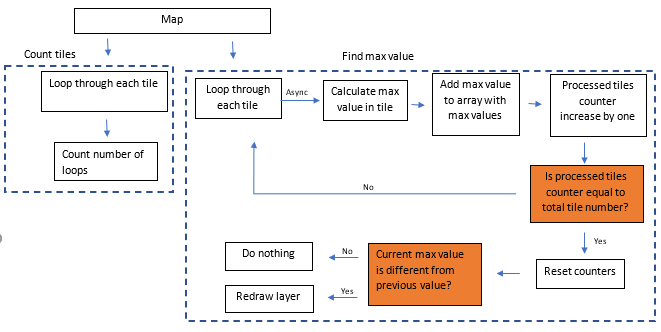
\includegraphics[width=.8\textwidth]{Pictures/DoubleLoop}
	\caption{Finding the largest value in all currently displayed tiles}
	\label{DoubleLoop}
\end{figure}

\section{Recolor when the max value change}

The recoloring function was already part of olGeoTiff. However, in Bernhard Baumrocks’ thesis this recoloring was triggered manually by the user when changing the color sliders. In this project the changing of colors will trigger automatically. The function for recoloring the map have therefore been set up to trigger, when the user stops changing the view. By not triggering before the map movement is finished a smoother user experience is ensured, since new tiles does not have to processed before the user is finished with interacting with the map. The recolor function is running through all of the code mentioned in the previous sections. 

\begin{lstlisting}[language=JavaScript, caption={The JavaScript in the project}, label= VoresJS,escapechar=|]
map.on("moveend", function() {
recolorMap()
});
});
\end{lstlisting}
\section{Polish}
In addition to the rendering of the raster in the map, some features were also added to improve the user experience.


\subsection{Two maps}

\begin{figure} [H]
	\centering
	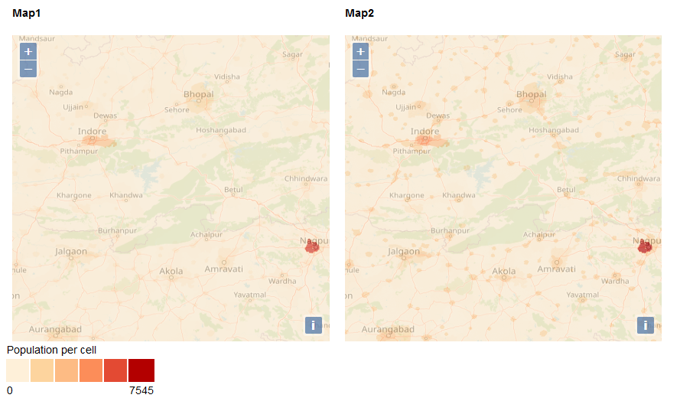
\includegraphics[width=.8\textwidth]{Pictures/DualMaps}
	\caption{A second map}
	\label{DualMaps}
\end{figure}
\fxnote{Update with a map, where the differences are more clear }
To be able to compare different rasters with each other a second map was added as illustrated in figure \ref{DualMaps}. This second map is having its own raster dataset but sharing the view with the first map. This means that the two maps would always show the same area. Panning or zooming in one map would do the same action in the other map. The two maps are sharing the same legend. 

The two projection are also sharing the same color scale. This means that the coloring is done based on the maximum value in the current extent of either of the maps. To accomplish this changes were made to the function, which were finding the maximum value among the tiles as illustrated in figure x.
 
\begin{figure} [H]
	\centering
	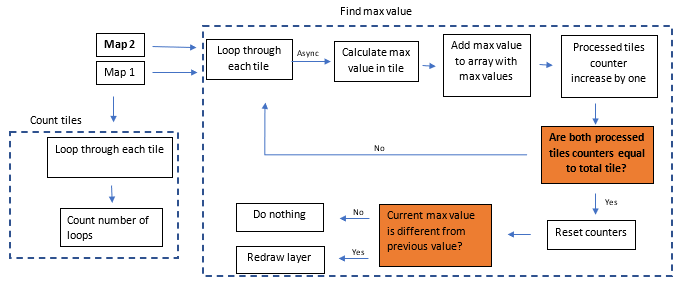
\includegraphics[width=.8\textwidth]{Pictures/ChangeToMaxCalculation}
	\caption{Calculating the maximum value for two maps. Changes from the original have been written in bold}
	\label{ChangeToMaxCalculation}
\end{figure}

This function is now being used twice, once for each layer. If the same function as presented in section x was used, then the redrawing would potentially trigger twice. 

To avoid this each of the maps are given their own processed tiles counter. The if statement, which is resetting the counters and triggering the recoloring, has been changed, so that it now is checking if both of these processed tiles counters is equal to the total number of tiles. Thereby the recoloring can only happen, when the tile in both maps have been processed. 

The two maps would always display the same amount of tiles, since they are sharing the same view. It is therefore only necessary to calculate the amount of tiles for one of the layers. 
%Add to dualmaps how the double evaluation for multiple maps were build 

\subsection{Search function}
In order to be able to faster navigate the map a search function was created as shown in figure \ref{SearchBar}. 

\begin{figure} [H]
	\centering
	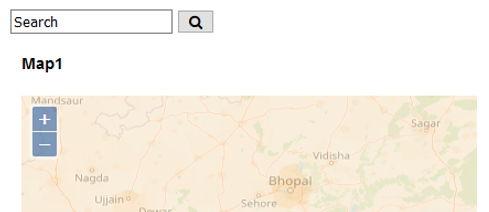
\includegraphics[width=.8\textwidth]{Pictures/SearchBar}
	\caption{The map can pan to a specific area, by searching for that area in the searchbar}
	\label{SearchBar}
\end{figure}

The user can use this to change the current view of the maps to a given location. This is accomplished through the help of Nominatim. This tool can search through Openstreetmap data by location names. It then returns data about the searched location. 

Among this data is the latitude and longitude for the central point of the place. \citep{Nominatim}
This coordinate is then used as the coordinate for the center of the map.
